\begingroup
% 11.1 TeX points keeps body/caption glyphs above 11 PDF points after conversion.
\renewcommand{\normalsize}{\fontsize{11.1pt}{13.3pt}\selectfont}
\normalsize
\captionsetup{font=normalsize}
\section{Question 1: Data Characteristics and Resource Imbalance}
\label{sec:q1}
\subsection{Data Characteristics}
The competition's adapted Alibaba trace contains \QOneJobs{} jobs and \QOneNodes{} nodes, providing \QOneGpus{} GPUs and \QOneCpus{} vCPUs across \QOneModels{} models. Required fields have no missing values or duplicate identifiers. We retain fractional CPU requests. Each job $j$ has submission time $r_j$, duration $d_j$ (seconds), and $W_j$ identical workers, each requesting $g_j$ GPUs and $c_j$ vCPUs. Requests are per worker; multiplying by $W_j$ gives the whole-job demand. Node capacities are treated as fixed. The supplied records contain requests rather than measured hardware activity; GPU names alone do not identify training, inference or application compatibility.

Most jobs are small by worker count: \QOneSingleWorkerPct\% have one worker, and \QOneOneGpuPct\% request one GPU per worker; the corresponding means are \QOneMeanWorkers{} and \QOneMeanWorkerGpus{}. Duration is highly dispersed: the median is \QOneMedianDuration{} s, the 95th percentile \QOnePninetyfiveDuration{} h, and the maximum approximately \QOneMaxDurationDays{} days. Thus a typical job poorly represents the long-duration tail.

Define full-lifetime GPU work as $H_j=W_jg_jd_j$ in GPU-seconds; $H_j/3600$ gives GPU-hours. Total work is \QOneWorkMillion{} million GPU-hours, with empirical Gini \QOneGini{}. Using $k=\lfloor f|\mathcal{J}|\rfloor$, the top 1\% (\QOneTopOneCount{} jobs) and 5\% (\QOneTopFiveCount{}) account for \QOneTopOneShare\% and \QOneTopFiveShare\% of work. Figure~\ref{fig:q1} shows concentration and duration tails; neither establishes a fitted power law. Queueing experiments must test whether these large jobs obstruct smaller arrivals.

\begin{figure}[!ht]
\centering
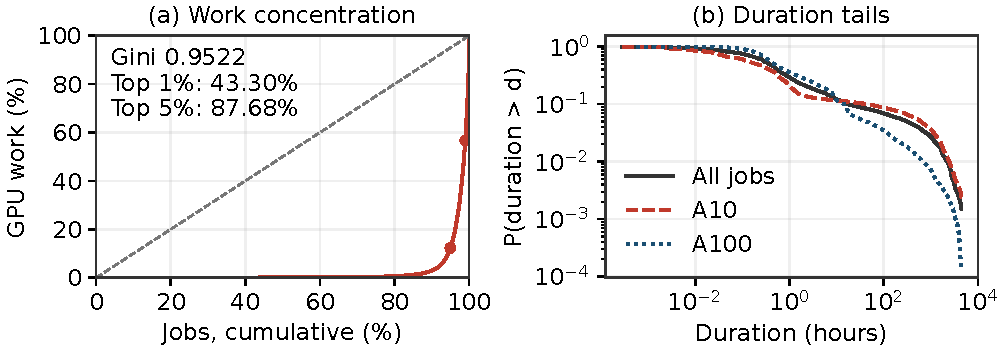
\includegraphics[width=\textwidth]{fig1_data_patterns.pdf}
\caption{(a) GPU-work Lorenz curve, including the origin; top-$k$ counts use floor rounding. (b) Strict empirical duration CCDF, $\Pr(d_j>x)$, with ties grouped; terminal zero is omitted on log axes. A100 denotes A100-SXM4-80GB.}
\label{fig:q1}
\end{figure}

\subsection{Supply--Demand Imbalance}
Set $T=\max_j r_j=\QOneHorizon$ s (\QOneHorizonHours{} h), \QOneWindowDifference{} s short of nominal 90 days. For model $m$, compare all submitted lifetime work with its capacity over $[0,T)$:
\begin{equation}
\rho_m^{\mathrm{GPU}}=\frac{\sum_{j\in\mathcal{J}_m}W_jg_jd_j}{T\sum_{i\in\mathcal{I}_m}G_i^{\mathrm{cap}}},\qquad
\rho_m^{\mathrm{CPU}}=\frac{\sum_{j\in\mathcal{J}_m}W_jc_jd_j}{T\sum_{i\in\mathcal{I}_m}C_i^{\mathrm{cap}}}.
\label{eq:load_ratio}
\end{equation}
Both denominators use seconds, matching the numerators. Work extending beyond $T$ remains included. These ratios measure workload pressure, not observed utilization or proof of steady-state instability. Table~\ref{tab:q1_pool} identifies A10's disproportionate pressure.

\begin{table}[!ht]
\centering
\caption{Submitted lifetime work versus exact-window capacity. Work is in million GPU-hours; GPU-s1/s2 abbreviate GPU-series-1/2.}
\label{tab:q1_pool}
\label{tab:q1_summary} % Preserve references from the integration baseline.
\setlength{\tabcolsep}{5pt}
\begin{tabular}{lrrrrr}
\toprule
GPU model & GPUs & Jobs & Work (10$^6$ GPU-h) & $\rho^{GPU}$ & $\rho^{CPU}$\\
\midrule
\texttt{A10} & 2,494 & 111,284 & 11.119 & 2.064 & 0.391\\
\texttt{A100-SXM4-80GB} & 3,456 & 80,877 & 5.936 & 0.795 & 0.534\\
\texttt{GPU-series-1} & 1,558 & 9,643 & 3.892 & 1.156 & 0.590\\
\texttt{H800} & 1,752 & 4,716 & 2.203 & 0.582 & 0.540\\
\texttt{GPU-series-2} & 976 & 13,633 & 1.224 & 0.580 & 0.382\\
\texttt{A800-SXM4-80GB} & 176 & 3,959 & 0.232 & 0.611 & 0.527\\
\textbf{Total} & 10,412 & 224,112 & 24.606 & 1.094 & 0.473\\
\bottomrule
\end{tabular}

\end{table}

To distinguish lifetime work from window overlap, define counterfactual immediate-start demand:
\begin{equation}
D_m(t)=\sum_{j\in\mathcal{J}_m}W_jg_j\mathbf{1}\{r_j\leq t<r_j+d_j\},\qquad
\overline{D}_m=\frac{1}{T}\int_0^T D_m(t)\,dt.
\label{eq:q1_demand}
\end{equation}
This assumes submission-time starts and ignores capacity. Exact event integration gives A10 a mean of \QOneAtenMean{} GPUs against \QOneAtenCapacity{} available, with an instantaneous peak of \QOneAtenPeak{}. The mean excess of \QOneAtenExcess{} GPUs is not a sufficient expansion prescription: CPU, node placement and temporal overlap also matter. Lower mean demand elsewhere does not guarantee spare capacity at every instant.

\begin{figure}[!ht]
\centering
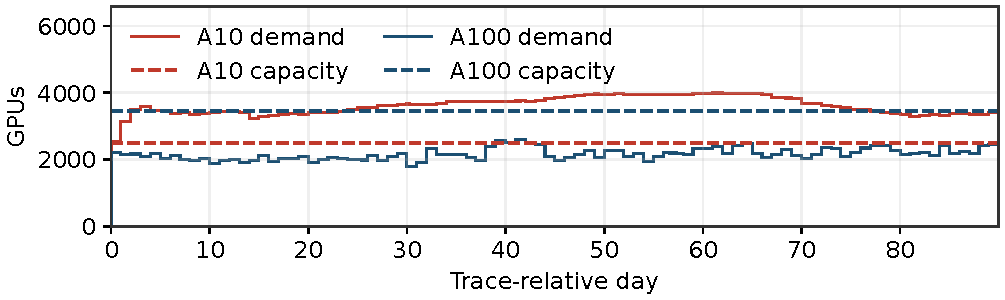
\includegraphics[width=\textwidth]{fig1_demand.pdf}
\caption{Counterfactual immediate-start demand, displayed as exact daily overlap averages. Dashed lines show physical capacity. Daily averaging hides instantaneous peaks; these curves are not actual allocation.}
\label{fig:q1-demand}
\end{figure}

All nodes are initially idle. The \QOneOriginJobs{} submissions at $r_j=0$ are the trace-origin batch, not already running services. Excluding that batch, exposure-corrected arrival rates differ by \QOnePhaseRatio{} times between relative 24-hour phases \QOnePhasePeak{} and \QOnePhaseTrough{}. With no calendar origin or timezone, these phases cannot identify afternoon or night peaks. Supplementary plots show daily arrivals, submitted work and the full phase profile. Work grouped by submission day includes each job's entire future duration; it is not work executed that day.

\subsection{Bottleneck Hypotheses}
GPU-series-1 contains \QOneOneNodes{} nodes with $(1\text{ GPU},192\text{ vCPUs})$, \QOneOneSmallNodes{} with $(1,128)$, \QOneFourNodes{} with $(4,192)$, and \QOneEightNodes{} with $(8,192)$. A pool-average CPU/GPU ratio obscures these configurations. Exactly \QOneHighRatioJobs{} jobs (\QOneHighRatioPct\%; \QOneHighRatioWorkPct\% of pool work) exceed the 8-GPU nodes' \QOneRatioThreshold{} vCPU/GPU ratio. One 192-vCPU, 1-GPU worker can exhaust such a node's CPUs while leaving seven GPUs unavailable to positive-CPU workers. This illustrates a possible placement mechanism, not a measured schedule.

The evidence motivates testing head-of-line blocking, node-ratio-aware placement and explicitly compatible cross-model capacity. Questions 2--3 must evaluate waiting, allocation and fairness with capacity-valid schedules. Q1 supports these hypotheses, but proves neither their causal effects nor any scheduler's optimality.
\par\endgroup
